\documentclass[uplatex]{jsarticle}

%% Packages
\usepackage[dvipdfmx]{graphicx,color,hyperref}
\usepackage{algorithm}
\usepackage{algorithmic}
\usepackage{url}
\usepackage{lscape}
\usepackage{mathtools}
\usepackage{here}
\usepackage{amsmath,amssymb,amsfonts}
\usepackage{amsthm}
\usepackage{tikz}
\usepackage{tcolorbox}
\usepackage{pxjahyper}

%% Theorem Styles
\newtheorem{theorem}{定理}
\newtheorem{proposition}{命題}
\newtheorem{cor}{系}
\newtheorem{definition}{定義}
\newtheorem{problem}{問題}
\theoremstyle{remark}
\newtheorem{remark}{注意}
\newtheorem{requirement}{条件}

%% Environment (Colorful Box)
\newenvironment{background}[1]{
    \begin{tcolorbox}[
        fonttitle=\bfseries,
        title={#1}
    ]
}{
    \end{tcolorbox}
}

\newenvironment{method}[1]{
    \begin{tcolorbox}[
        colframe=green!50!black,
        colback=green!50!black!10!white,
        colbacktitle=green!50!black!40!white,
        coltitle=black,
        fonttitle=\bfseries,
        title={#1}
    ]
}{
    \end{tcolorbox}
}

\newenvironment{experiment}[1]{
    \begin{tcolorbox}[
        colframe=violet,
        colback=violet!10!white,
        colbacktitle=violet!40!white,
        coltitle=black,
        fonttitle=\bfseries,
        title={#1}
    ]
}{
    \end{tcolorbox}
}

%% Title
\title{Break the Sequential Dependency of LLM Inference Using Lookahead Decoding}
\author{\empty}
\date{\empty}

%% Document body
\begin{document}
\maketitle

\begin{itemize}
    \item Link: \url{https://dl.acm.org/doi/10.5555/3692070.3692631}
    \item Conference: ICML2024
    \item Citation: \cite{lookahead_decoding}
    \item コード: \url{https://github.com/hao-ai-lab/LookaheadDecoding}
\end{itemize}

\section{概要}
\begin{tcolorbox}[fonttitle=\bfseries]
大規模言語モデルの自己回帰型のデコーディングは、メモリ帯域幅によって制限されており、これが大きなレイテンシの原因となっている。また逐次的にデコーディングするため最新のアクセラレータの並列処理能力をうまく使えていない。LLMのデコーディングを高速化するための既存の手法(e.g. 投機的デコーディング)は、ドラフトモデル(補助モデル)を必要とするが、このモデルの入手は容易ではなく、汎用性もない。

本論文では、LOOKAHEAD DECODINGという、補助モデルやデータストアを必要とせずにLLMのデコーディングを高速化するデコーディングアルゴリズムを提案する。このアルゴリズムは、先読みしてでコーディングを行うLookahead branchとその出力がLLMの出力分布と一致するか確認するVerification branchを主な構成要素としており、それにより高速なデコーディングを可能とする。複数のアクセラレータ上で並列化が可能であることも特徴である。
LOOKAHEAD DECODINGの実装は、MT-benchで自己回帰デコーディングを最大1.8倍、コード補完タスクでは複数GPUを利用することにより最大4倍高速化できることを示した。

\end{tcolorbox}

\section{背景}
\begin{background}{Jacobi Decoding}
Jacobi decodingは非線形方程式の解法であるJacobi法にアイデアを得たものである。
大雑把な説明としては入力$x$に対して、ある初期値出力$y^0 \in \mathbb{N}^m$から初めて, 
$y_j^i = \mathrm{argmax} P_M(y_j| y_{1:j-1}^{i-1}, x)\ (j = i, i+1, \dots, m)$を繰り返して、$y^i$を次々に得ていくことでデコーディングを行う。上の式は各$j$について並列化可能であることが特徴である(\url{https://github.com/hao-ai-lab/LookaheadDecoding?tab=readme-ov-file#background-parallel-llm-decoding-using-jacobi-iteration}のアニメーションを見たほうがわかりやすい)。
\end{background}

\section{手法}
\begin{figure}
    \centering
    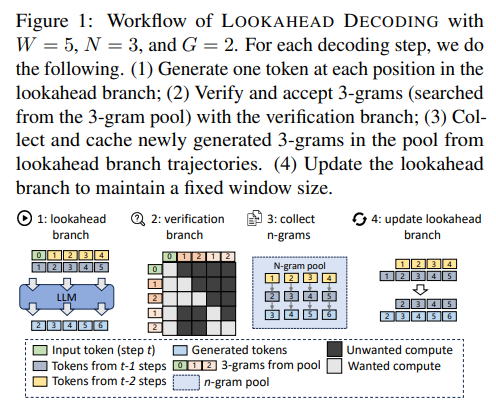
\includegraphics[width=0.5\textwidth]{img/lookahead_decoding/overview.png}
    \caption{Lookahead Decodingの概要図}
    \label{fig:overview}
\end{figure}

\begin{method}{Lookahead Decoding}
提案手法における重要な構成要素は
\begin{itemize}
    \item トークンウィンドウ$W$: $N \times W$の行列で、$N$は持つトークンの軌跡の数、$W$はウィンドウのサイズを表す。
    \item キャッシュ$C$: $n$-gramの出力候補を保存する($n = N$である)。
\end{itemize}
である。

\begin{enumerate}
    \item Lookahead branch: 入力、これまでの出力、ウィンドウ内のトークンを用いて、次のトークンの候補を生成する。
    \item Verification branch: キャッシュ$C$にある$n$-gramのうち、もっとも今の出力に続くものとして適合するものを選ぶ。
    \item Collect n-grams: Lookahead branchで得られた候補をキャッシュ$C$に追加する。
    \item Update lookahead branch: 次のステップのためにLookahead branchを更新する。これは最も時系列的に最も昔のトークンを消して、最新のトークンを追加することを意味する。
\end{enumerate}
上の四つのフェーズの説明は\url{https://github.com/hao-ai-lab/LookaheadDecoding?tab=readme-ov-file#lookahead-decoding-make-jacobi-decoding-feasible}のGIFがわかりやすい。
上の4つのフェーズを繰り返すことで、最終的な出力をアウトプットする。
\end{method}

\section{実験}
\begin{experiment}{実験1}
\ref{fig:template}のように図を引用することができる.
\end{experiment}

\begin{figure}
    \centering
    
\includegraphics[width=0.5\textwidth]{img/image.png}
    \caption{キャプション}
    \label{fig:template}
\end{figure}

\section{感想}
\begin{tcolorbox}[colframe=brown,
  colback=brown!10!white,
  colbacktitle=brown!40!white,
  coltitle=black,fonttitle=\bfseries]
\begin{itemize}
    \item 正直難しくて雰囲気しかわからず、よくわからないところが多い。
\end{itemize}
\end{tcolorbox}

% \section{MEMO}
% ここはコンパイルするときにコメントアウトする!!
% \begin{itemize}
%     \item Attention特にCausal attentionの説明
%     \item Autoregressive LLMの動き方
%     \item Jacobi decoding -> あまりうまくいかない、違う場所にtokenが置かれることが多い
% \end{itemize}
% \subsection{Abstract}
% 大規模言語モデル(LLM)の自己回帰デコーディングは、メモリ帯域幅によって制限されており、これが高いレイテンシ(遅延)と、最新のアクセラレータの並列処理能力の著しい浪費につながっています。LLMのデコーディングを高速化するための既存の手法(例:投機的デコーディング)は、ドラフトモデル(補助モデル)を必要としますが、このモデルの入手は容易ではなく、汎用性もありません。

% 本論文では、LOOKAHEAD DECODINGという、補助モデルやデータストアを必要とせずにLLMのデコーディングを高速化する、正確で並列なデコーディングアルゴリズムを提案します。このアルゴリズムは、ステップあたりの計算量(log(FLOPs))を増やすことで、デコーディングの総ステップ数を削減することを可能にします。また、単一または複数の最新のアクセラレータ上でより並列化が可能であり、メモリ効率の良い注意機構(例:FlashAttention)とも互換性があります。

% 我々のLOOKAHEAD DECODINGの実装は、MT-benchで自己回帰デコーディングを最大1.8倍、コード補完タスクでは複数GPUでの強力なスケーリングにより最大4倍高速化できることを示しました。

% コードはこちらで公開されています: https://github.com/hao-ai-lab/LookaheadDecoding

% \subsection{2 Background}
% このセクションでは、自己回帰デコーディングとヤコビデコーディングの両方を、非線形システムを解くという観点から定式化します。

% \subsubsection{デコーダモデルにおける因果的アテンション}

% 今日の大規模言語モデル (LLM) のほとんどは、主に2つの要素で構成されています。一つはトークン単位のモジュール(MLPや正規化層を含む)、もう一つはアテンションモジュールです。

% アテンションモジュール内ではトークン同士が相互作用しますが、その他のトークン単位のモジュールでは、トークンは互いに情報をやり取りすることなく処理されます。

% アテンション層は、クエリ (Q)、キー (K)、バリュー (V) という3つの入力要素で構成され、それぞれの i番目のトークンは
% $Q_i, K_i, V_i$と表記されます。

% アテンション層は次の演算を実行します: $O = softmax(QK^\top)V$.

% デコーダモデル特有の因果的アテンションでは、$QK^\top$
%   に下三角マスクが適用されます。これにより、$O_i$
%   (出力$O$の$i$番目のトークン)は、$Q_i$
%   と, $j \leq i$ である $K_j$
%   および $V_j$
%   からのみ計算されることが保証されます。

% LLM内の他のすべての層がトークン単位の操作を実行するため、任意のモデル入力$x$と出力$o$に対して、$o_i$
%   (出力$o$の$i$番目のトークン)は、$j\leq i$である$x_j$
%   (入力$x$の$j$番目のトークン)によってのみ影響を受けます。

% \subsubsection{LLMにおける自己回帰デコーディング}
% これまでの出力と入力から一個ずつ推論する

% \subsubsection{Guess-And-Verify Paradig}
% 一個ずつではなくて数個ずつ推論する。数個ずつDraft modelで推論して、LLMで
% それを並列に検証する。検証結果と一致していればそのまま進めて、そうでなければそこからやり直す。

% \subsubsection{Jacobi decoding}
% Autoregressiveなdecodingを非線型方程式とみなして
% それをJacobi法で解くことで解を求める。
% Q微分できなくね??前の論文ちゃんと読まないとわからなさそう。
% Qn-gramがどうのこうのみたいなのがわからない。
% なんかアルゴリズムを見るとわかりそう。
% Algorithm1

% \subsubsection{Limitations of Jacobi decoding}

% \subsection{3 Lookahead Decoding}
% \begin{enumerate}
%     \item Lookahead branch; jacobiを回す
%     \item Verification branch; jacobiで得られたいくつかの候補がLLM distributionと一致するか確かめる
%     \item Collect n-grams; いい感じのn-gramを選ぶ
%     \item Update lookahead branch; 次ステップのためにbranchをupdate
% \end{enumerate}
% 説明はいろいろ書いてあるが、正直以下のやつが一番わかりやすい。
% \url{https://github.com/hao-ai-lab/LookaheadDecoding?tab=readme-ov-file#lookahead-decoding-make-jacobi-decoding-feasible}

% まずベーシックなもの

% \begin{itemize}
%     \item + Verificationをサンプリングでやる
%     \item + attention maskってなに?見れる見れないの話がよくわからん。
%     \item + FlashAttentionの導入による実装上の高速化
%     \item + VerificationとLookaheadの並列化
% \end{itemize}

% \subsection{4 Scaling law of Lookahead Decoding}
% \subsection{5 Evaluation results}


\bibliographystyle{jplain}
\bibliography{template.bib}

\end{document}